\documentclass[12pt, a4paper]{article}

\usepackage [utf8]{inputenc}
\usepackage [IL2]{fontenc}
\usepackage [czech]{babel}
\usepackage{graphicx}
\usepackage[numbib]{tocbibind}
\usepackage{hyperref}
\graphicspath{{d:/yyy/}}
\newcommand{\Break}{\State \textbf{break} }

\title{
\includegraphics[width=10cm]{FAV_cmyk}

{\huge Semestrální práce z KIV/TI}

\vspace{0.5cm}
{\LARGE Logické řízení - sanitace nádrží}
\vspace{1cm} 

\Large Lukáš Runt (A20B0226P), Miroslav Vdoviak (A20B....)
\vspace{0.5cm} 

\large \itshape lrunt@students.zcu.cz, lrunt@students.zcu.cz
}
\date{\vspace{6cm} \today}

\begin{document}

\begin{titlepage}
\clearpage\maketitle
\thispagestyle{empty}
\end{titlepage}
\tableofcontents \newpage

\section{Zadání}

\section{Analýza úlohy}

\section{Automatový model}

\section{Implementace}

\newpage
\section{Uživatelská příručka}

\subsection{Spuštění programu}
Před spuštěním programu musíme nejprve zkontrolovat, zda se nacházíme ve stejné složce, jako je právě soubor semestralkaTI.jar. Tento program spustíme v příkazové řádce příkazem: \texttt{java -jar semestralkaTI.jar}. Pro spuštění je předpokladem mít nainstalovanou javu verze nejméně 11.

\begin{figure}[h]
\centering 
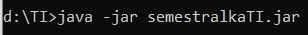
\includegraphics{prikladSpusteni}
\caption{Příklad spuštění}
\end{figure}

Pokud se program podaří spustit zobrazí se model sanitarizace tanků.

\begin{figure}
\centering 
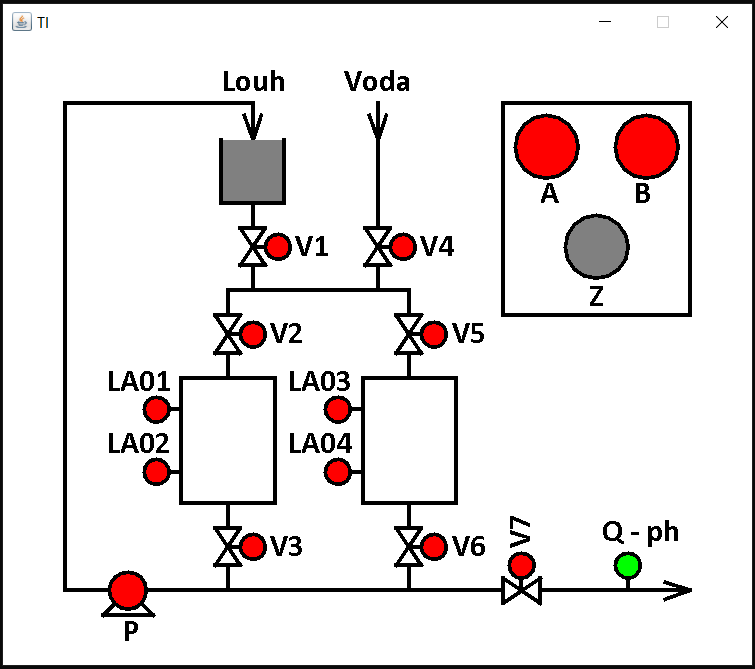
\includegraphics[width=10cm]{vzhledAplikace}
\caption{Vzhled aplikace po spuštění}
\end{figure}

\subsection{Ovládání}
Program se ovládá pomocí klávesnice: \newline 
A - Spuštění sanitarizace tanku A \newline 
B - Spuštění sanitarizace tanku B \newline 
P - Manuální spuštění čerpadla \newline 
1 - Manuální otevření ventilu 1 \newline 
2 - Manuální otevření ventilu 2 \newline 
3 - Manuální otevření ventilu 3 \newline 
4 - Manuální otevření ventilu 4 \newline 
5 - Manuální otevření ventilu 5 \newline 
6 - Manuální otevření ventilu 6 \newline 
7 - Manuální otevření ventilu 7 \newline 


\section{Závěr}
Celkovou práci hodnotím pozitivně, neboť jsem si vyzkoušel napsat konečný automat. Byl to pro mne nepopsatelný zážitek, který mě studijně obohatil a posunul o krok blíže k praktickým aplikacím teoreticky získaných vědomostí. 

\end{document}